\begin{figure}
    \centering
    \begin{subfigure}{\linewidth}
        \centering
        \inputminted{c}{code/hello_world_kernel.c}
        \caption{CUDA code to be compiled by \mintinline{c}{nvcc}.
        Note differences \mintinline{c}{__global__} and \mintinline{c}{matrix_sum<<m,n>>} from standard C.}
        \label{lst:cuda_hello_world}
    \end{subfigure}
    \\[3ex]
    \begin{subfigure}{\linewidth}
        \centering
        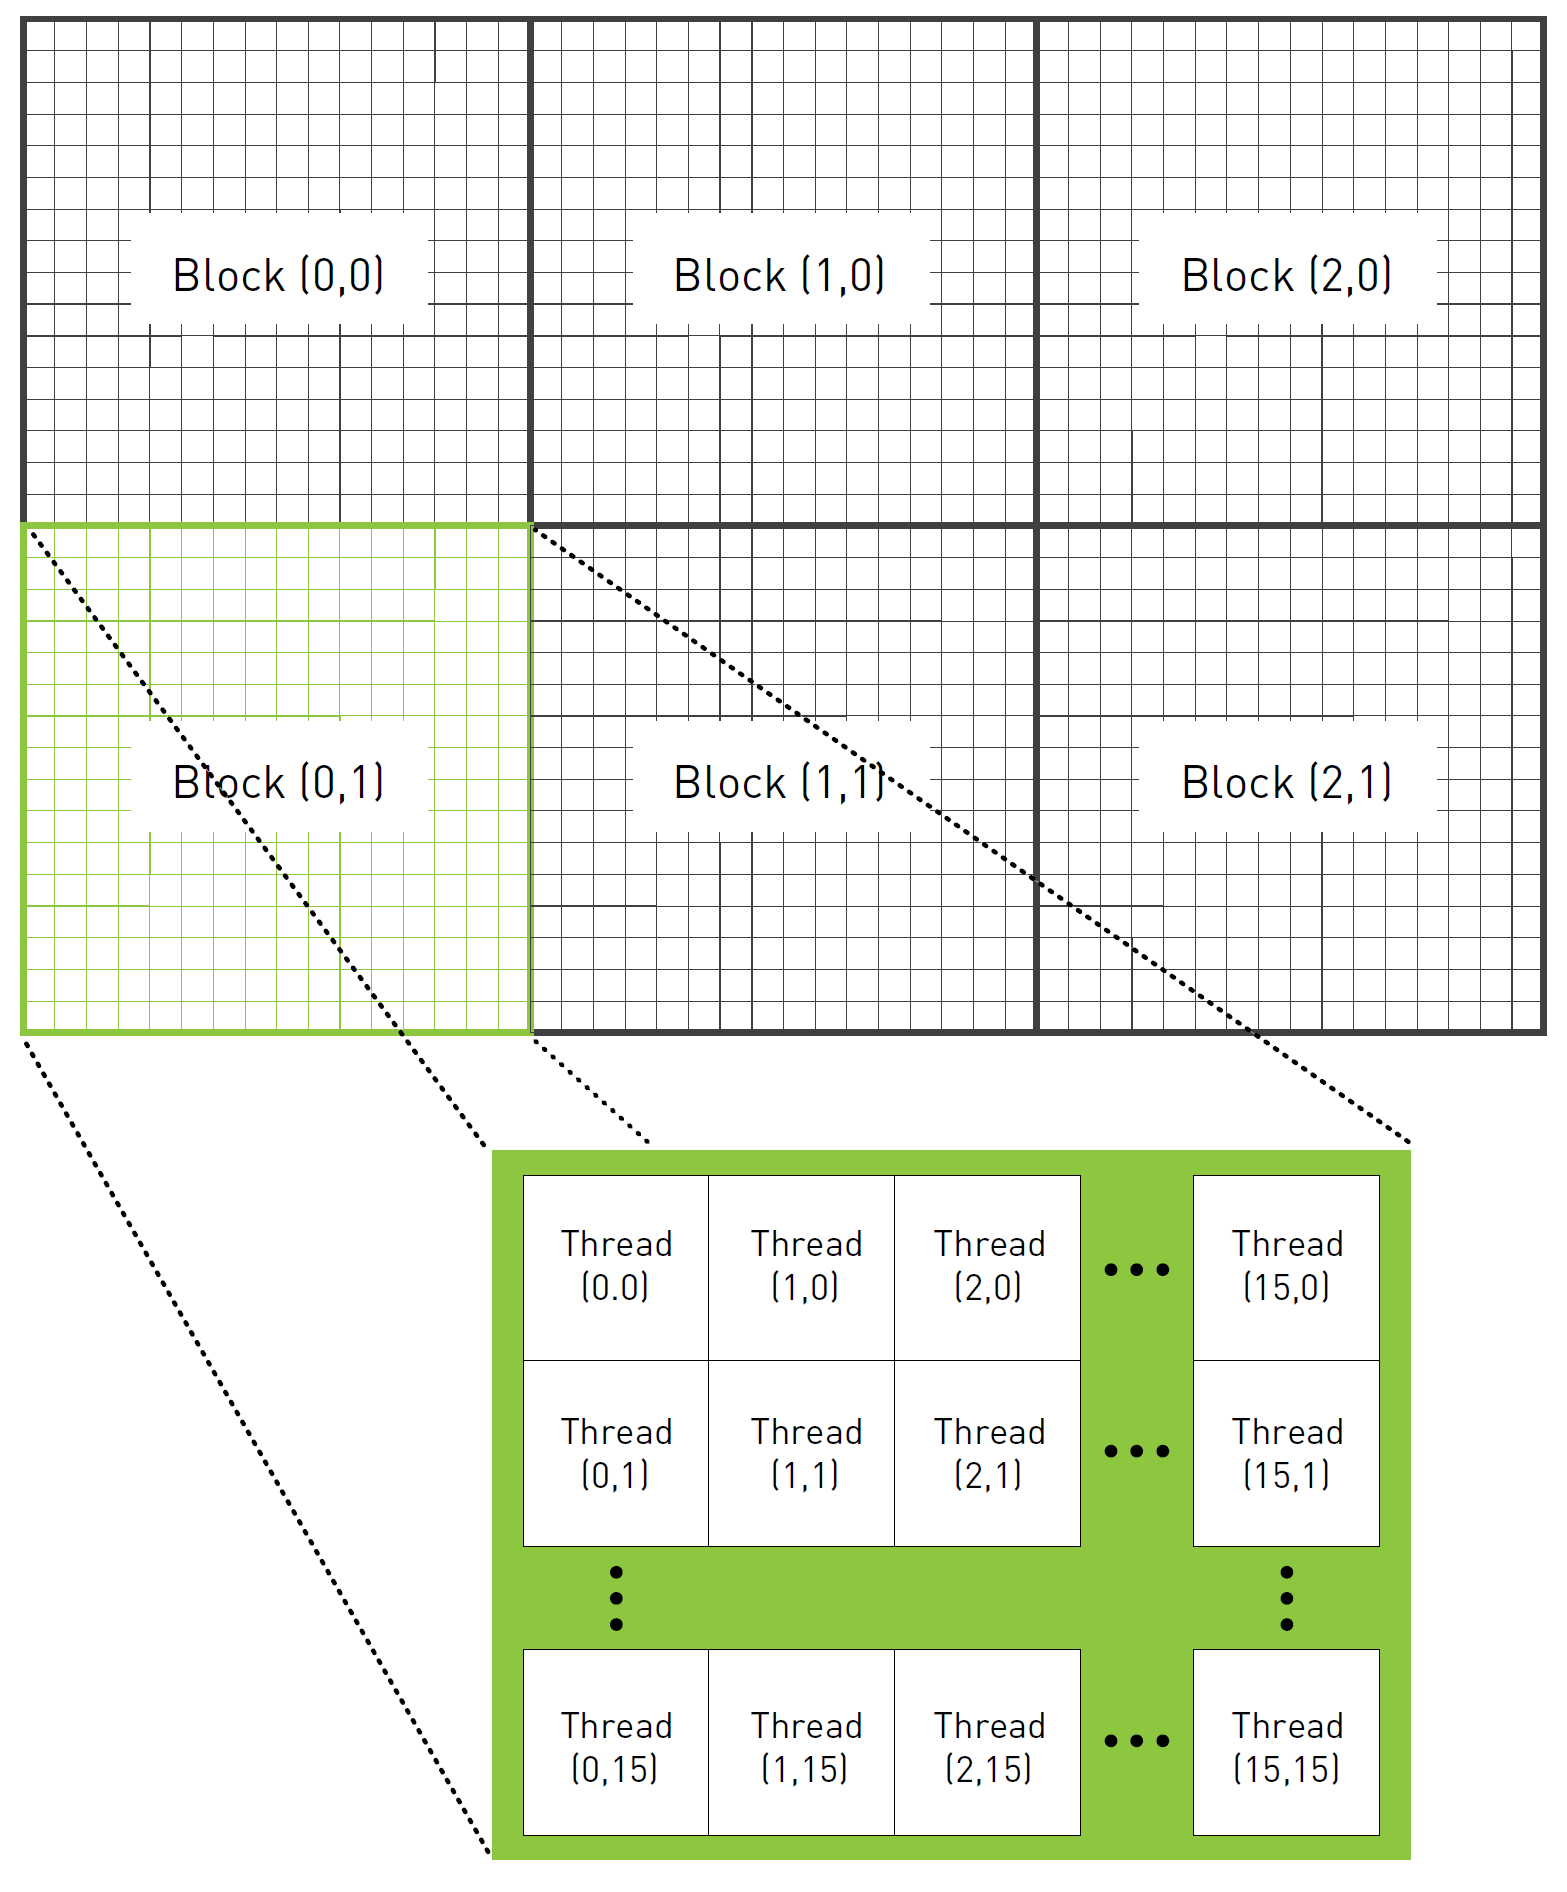
\includegraphics[width=.8\linewidth]{figures/matrix_thread.png}
        \caption{Mapping from thread and block to matrix element.}
        \label{fig:matrix_thread}
    \end{subfigure}
    \caption{Canonical CUDA "Hello world" kernel (matrix addition).}
    \label{fig:cuda_hello_world}
\end{figure}
